\section{Comunidade acadêmica}
\label{s.community}

\begin{frame}{Comunidade acadêmica}
	\justify 
	\begin{itemize}
		\item<1> Grupo de pessoas de instituições de ensino superior as quais engajam-se em atividades ``intelectuais", tais como \textbf{ensino}, \textbf{aprendizado} e \textbf{pesquisa};
		\\~\\
		\item<2> Comunidade deve ser \textbf{inclusiva}, \textbf{diversa} e \textbf{abrangente}, não limitando a participação de quaisquer pessoas;
		\\~\\
		\item<3> Como garantir que as pesquisas sejam ``honestas"~e sigam um conjunto de \textbf{boas práticas}?
	\end{itemize}
\end{frame}

\begin{frame}{}
	\centering
	\begin{figure}
		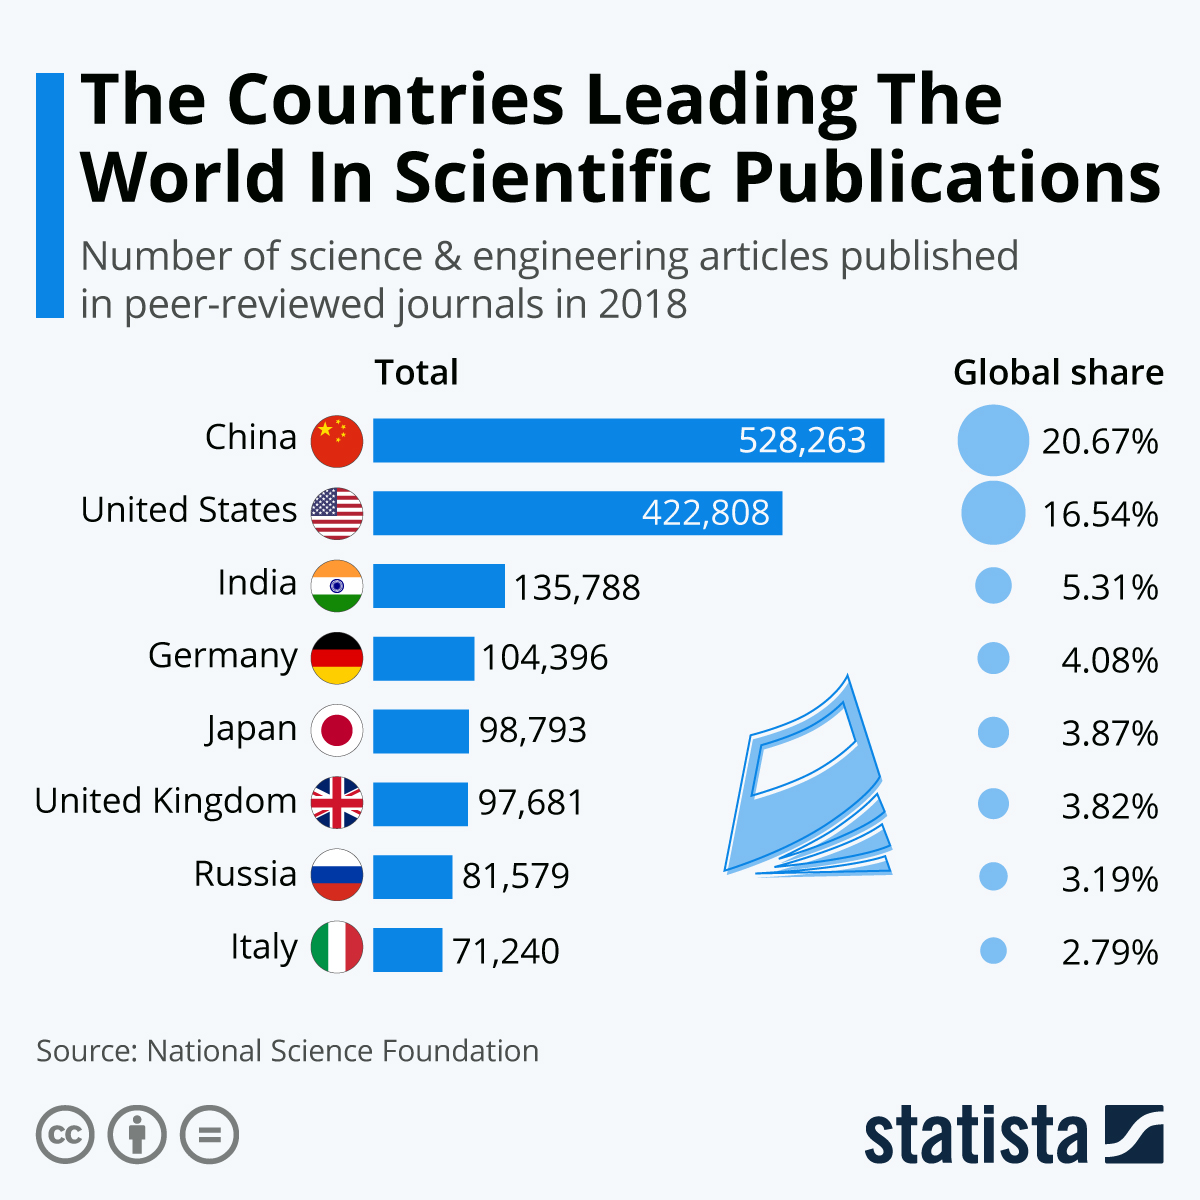
\includegraphics[scale=0.125]{figs/lead_country_papers.png}
		\caption{Ranking de países líderes em publicações nas áreas de Ciência e Engenharia no ano de 2018~\cite{Statista:18}.}
		\label{f.lead_country_papers}
	\end{figure}
\end{frame}

\subsection{Reprodutibilidade e integridade}
\label{ss.reproducibility_integrity}

\begin{frame}{Reprodutibilidade e integridade}
	\begin{block}{\centering Reprodutibilidade}
		Pesquisa deve ser passível de reprodução pela comunidade a partir da leitura do artigo e da utilização de ferramentas disponibilizadas.
	\end{block}
	\vspace{1cm}
	\begin{block}{\centering Integridade}
		Pesquisa deve ser íntegra, ou seja, os autores devem reportar honestamente o objetivo, metodologia e resultados obtidos.
	\end{block}
\end{frame}

\subsection{Impacto social}
\label{ss.social_impact}

\begin{frame}{Impacto social}
	\justify 
	\begin{itemize}
		\item<1> Existem \textbf{diversos fatores} que contribuem para o \textbf{``sucesso"}~de uma pesquisa;
		\\~\\
		\item<2> O processo de pesquisa \textbf{não} pode ser exclusivamente \textbf{dependente} de \textbf{métricas}, tais como, visibilidade, citações, dentre outras;
		\\~\\
		\item<3> \textbf{Inúmeras} pesquisas contribuem mais com \textbf{impactos sociais} do que com impactos acadêmicos.
	\end{itemize}
\end{frame}

\begin{frame}{}
	\centering
	\begin{figure}
		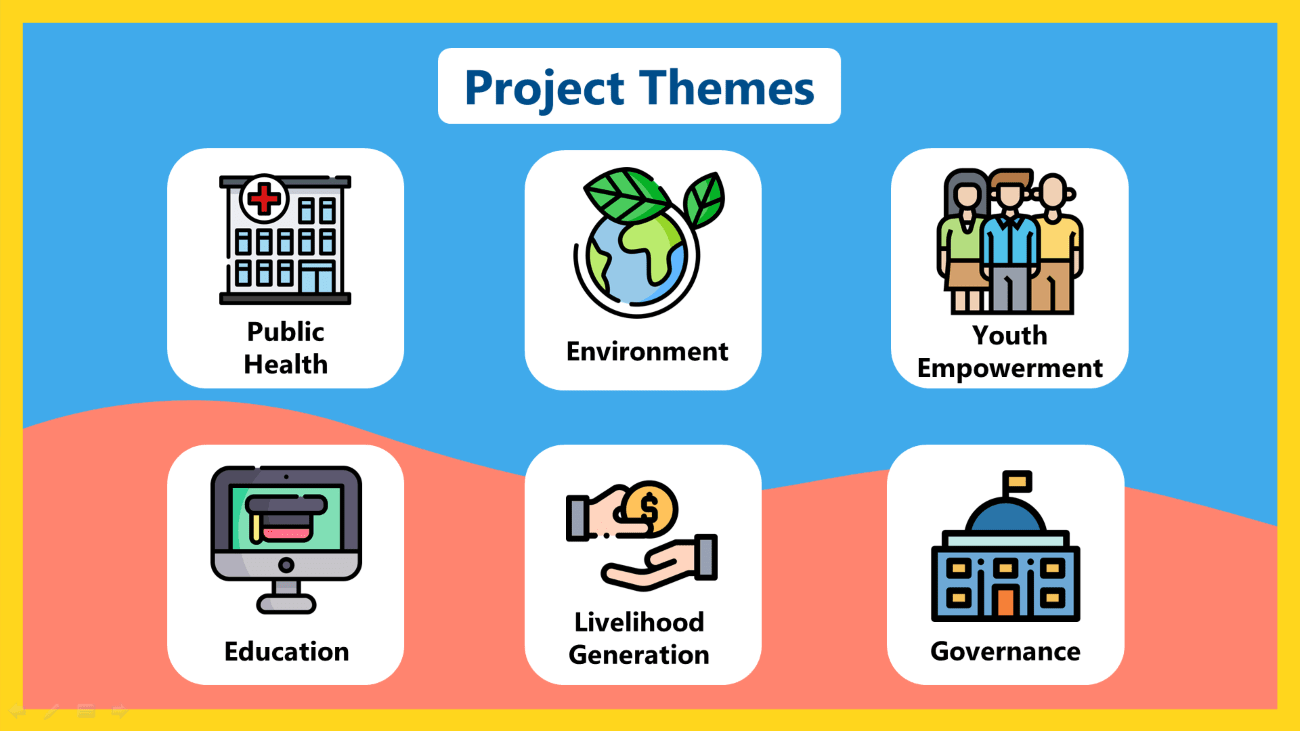
\includegraphics[scale=0.2]{figs/social_impact_research.png}
		\caption{Exemplos de áreas que beneficiam-se com o impacto social das pesquisas~\cite{YLAC:21}.}
		\label{f.social_impact_research}
	\end{figure}
\end{frame}
